\usetikzlibrary {petri,positioning}
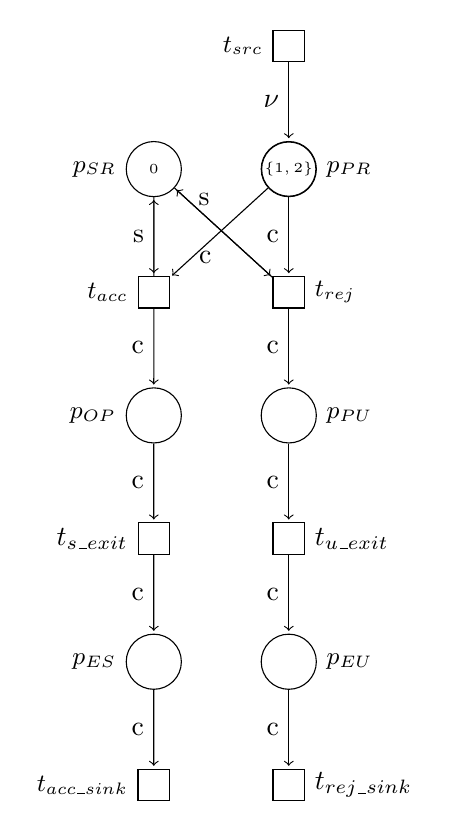
\begin{tikzpicture}[scale=0.7]
\centering

%source transition
\node[transition,minimum height=.4cm,minimum width=.4cm,label=left:{\small $t_{src}$}] (t0) {};

		
%parking requested client place
\node[place,label=right:{\small $p_{PR}$},minimum height=.70cm, minimum width=.5cm,below=of t0] (p0) {} 
edge[pre] node[auto] {$\nu$} (t0);
\node[token,fill = white, minimum height=0.40cm, minimum width=.5cm,draw=black,text=black] at (p0) {\text{$\{1,2\}$}};
		
		%server ready place			
		\node[place,label=left:{\small $p_{SR}$},minimum height=.70cm, minimum width=.5cm,left=of p0] (p1){};
\node[token,fill = white, text=black] at (p1) {$0$};

%places and transitions for request granted scenarios		
		%accept transition
		\node[transition,minimum height=.4cm,minimum width=.4cm,label=left:{\small $t_{acc}$}, below=of p1] (t1){}
		edge[pre] node[auto] {s} (p1)
		edge[post] node[auto] {} (p1)
		edge[pre] node[xshift=-5pt, yshift=-9pt] {c} (p0);
		%edge[post] node[auto] {} (p0);
		
	
		%client place occupy parking lot op
		\node[place,label=left:{\small $p_{OP}$},minimum height=.70cm, minimum width=.5cm,below=of t1] (p2){}
		edge[pre] node[auto] {c} (t1) ;	
		

		%transition exit successfully
		\node[transition,minimum height=.4cm,minimum width=.4cm,label=left:{$t_{s\_exit}$},below=of p2] (t2){}
		edge[pre] node[auto] {c} (p2);
		
		%client place Exit successfully ES
		\node[place,label=left:{\small $p_{ES}$},minimum height=.70cm, minimum width=.5cm,below=of t2] (p4){}
		edge[pre] node[auto] {c} (t2);			

		
		%transition accept sink
		\node[transition,minimum height=.4cm,minimum width=.4cm,label=left:{\small $t_{acc\_sink}$},below=of p4] (t3) {} edge[pre] node[auto] {c} (p4) ;
		
%request rejected scenarios		
		
		%reject transition
		\node[transition,minimum height=.4cm,minimum width=.4cm,label=right:{\small $t_{rej}$},below=of p0] (t4){}
		edge[pre] node[xshift=-7pt,yshift=12pt] {s} (p1)
		edge[post] node[auto] {} (p1)
		edge[pre] node[auto] {c} (p0);
		%edge[post] node[auto] {} (p0);


		%client place parking unavailable PU
		\node[place,label=right:{\small $p_{PU}$},minimum height=.70cm, minimum width=.5cm,below=of t4] (p6){}
		edge[pre] node[auto] {c} (t4) ;

		% transition unsuccesful exit
		\node[transition,minimum height=.4cm,minimum width=.4cm,label=right:{$t_{u\_exit}$},below= of p6] (t5) {}
		edge[pre] node[auto] {c} (p6);

		%client place Exit unsuccessfully EU
		\node[place,label=right:{\small $p_{EU}$},minimum height=.70cm, minimum width=.5cm,below=of t5] (p7){}
		edge[pre] node[auto] {c} (t5) ;

		% transition reject sink
		\node[transition,minimum height=.4cm,minimum width=.4cm,label=right:{$t_{rej\_sink}$},below= of p7] (t5) {}
		edge[pre] node[auto] {c} (p7);


\end{tikzpicture}


